
\section*{Extended Data}
\vspace{2\baselineskip}

\begin{extendedfigure}[ht]
    \centering
    % Top horizontal rule
    \noindent\rule{\linewidth}{0.4pt}\par\vspace{6pt}
    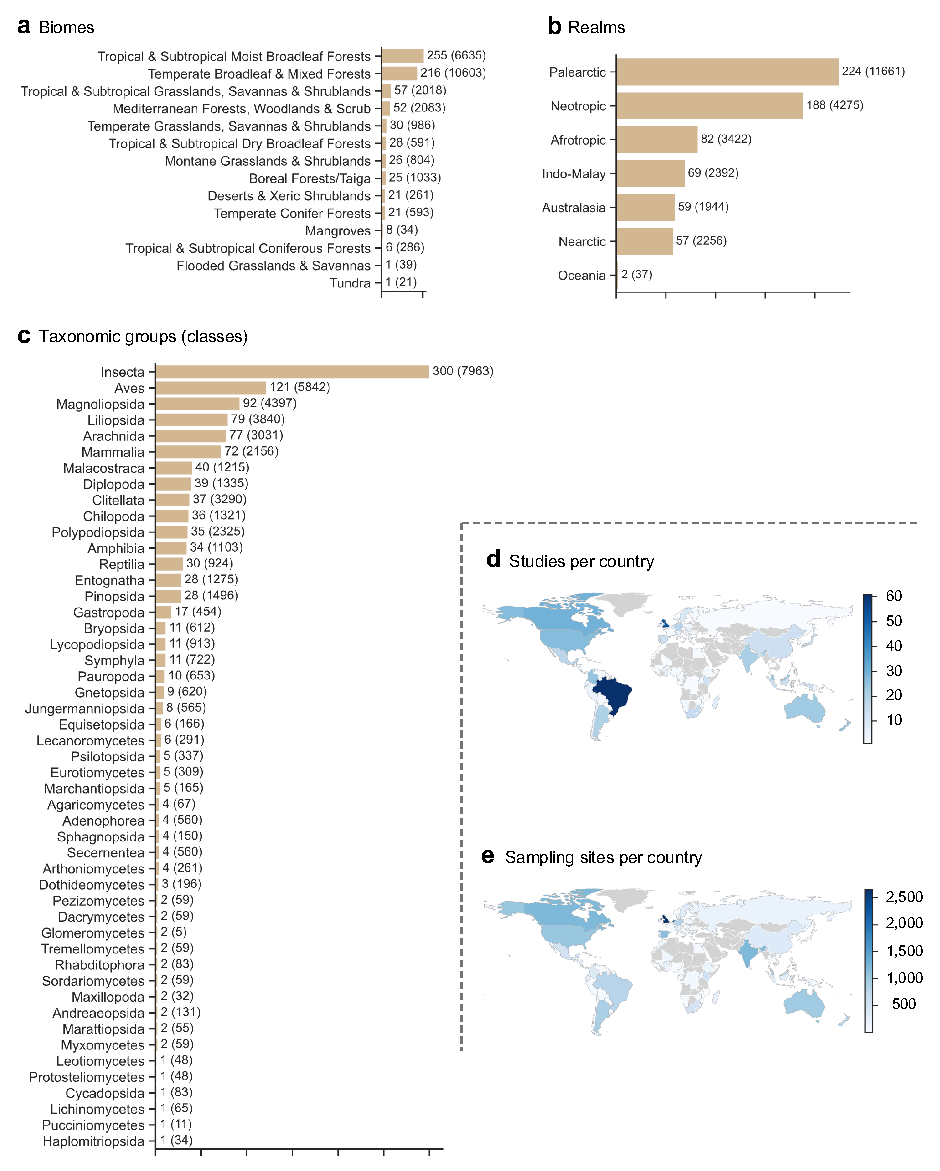
\includegraphics[width=0.95\linewidth]{figures/extended/predicts_data.pdf}
    \caption{
    \textbf{PREDICTS data coverage.}
    \textbf{a-c}, Number of source studies and sampling sites (in parenthesis) in the model data, split by biomes (\textbf{a}), realms (\textbf{b}), and taxonomic classes (\textbf{c}).
    \textbf{a,b}, Number of source studies (\textbf{a}) and sampling sites (\textbf{b}) per country in the data. Countries with no data are shown in grey.}
    \label{fig:predicts_data}
\end{extendedfigure}
\vspace{2\baselineskip}
\newpage

\begin{extendedtable}[ht]
  \centering
  \caption{\textbf{List of variables used across the different models}. These are divided into three categories: i) human impacts (used in all models), ii) environmental drivers (used in the BHMs), and iii) differences between site-pairs (used in the beta diversity models). The Haversine spatial distances are based on the sampling site coordinates from PREDICTS. The Gower environmental distance was calculated using the min and max temperature of the coldest and warmest month, the precipitation of the driest and wettest month, and elevation, all at the 1~km$^2$ scale. Repeated information from the row above is indicated by -.}
  \small
  \setlength{\tabcolsep}{7pt}
  \begin{tabular}{lcccc}
  \toprule
  Model variables & Spatial scale & Source & \makecell{Spatial\\resolution} & \makecell{Temporal\\resolution} \\
  \midrule
  \textit{i) Human impacts (all models)} & & & & \\
  \midrule
  Primary vegetation, light use & Sampling site & PREDICTS & Varying & Sampling date \\
  Primary vegetation, intense use & - & - & - & - \\
  Secondary vegetation, minimal use & - & - & - & - \\
  Secondary vegetation, light use & - & - & - & - \\
  Secondary vegetation, intense use & - & - & - & - \\
  Cropland, minimal use & - & - & - & - \\
  Cropland, light use & - & - & - & - \\
  Cropland, intense use & - & - & - & - \\
  Pasture, minimal use & - & - & - & - \\
  Pasture, light use & - & - & - & - \\
  Pasture, intense use & - & - & - & - \\
  Urban, all use intensities & - & - & - & - \\
  Mean population density (log) & 1, 50 km$^2$ & GPW & 1 km$^2$ & Yearly \\
  Mean road network density (log) & - & gROADS & Varying & Static \\
  \midrule
  \textit{ii) Environmental (BHMs)} & & & & \\
  \midrule
  Annual mean temperature & 1 km$^2$ & BioClim & 1 km$^2$ & 1970--2000 avg \\
  Temperature seasonality & - & - & - & - \\
  Annual precipitation & - & - & - & - \\
  Precipitation seasonality & - & - & - & - \\
  Elevation & 1, 10 km$^2$ & EarthEnv & 1 km$^2$ & Static \\
  Terrain roughness index & - & - & - & - \\
  \midrule
  \textit{iii) Site-site differences (beta models)} & & & & \\
  \midrule
  Difference in (log) population density & 1 km$^2$ & GPW & 1 km$^2$ & Yearly \\
  Difference in (log) road density & - & gROADS & Varying & Static \\
  Haversine spatial distance & n/a & \textit{Calculated} & n/a & n/a \\
  Gower environmental distance & - & - & - & - \\
  \bottomrule
\end{tabular}
  \label{tab:variables}
\end{extendedtable}
\newpage


\begin{extendedfigure}[H]
    \centering
    % Top horizontal rule
    \noindent\rule{\linewidth}{0.4pt}\par\vspace{6pt}
    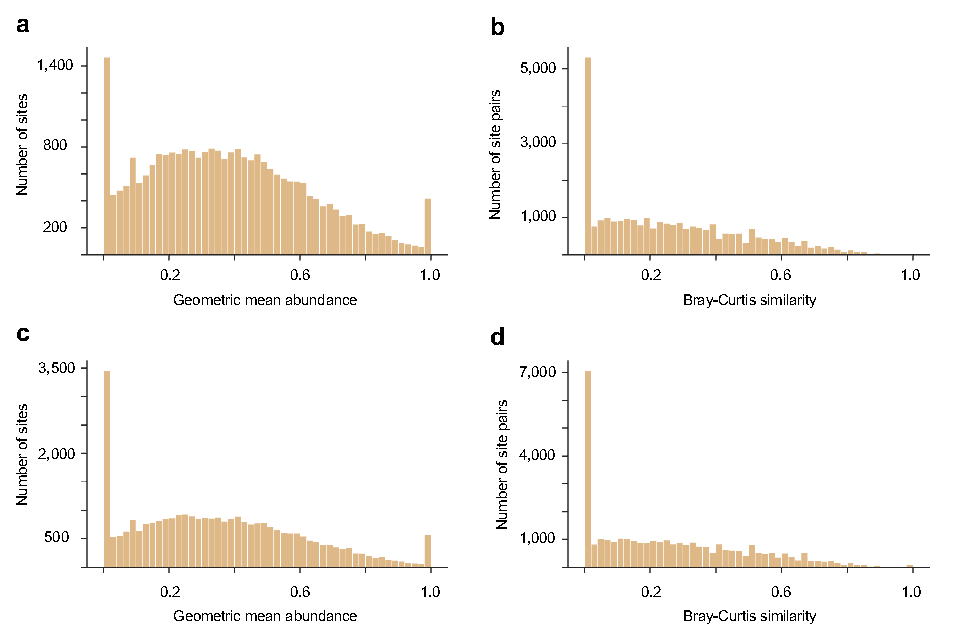
\includegraphics[width=0.95\linewidth]{figures/extended/response_variable_distr.pdf}
    \caption{
    \textbf{Response variable distributions.}
    Data distribution of the response variables for the alpha and beta diversity models. Alpha diversity is measured as the geometric mean abundance per site (for the SBM model, \textbf{a}) or per site and taxa (BTM model, \textbf{c}). Beta diversity is measured as the Bray-Curtis similarity between pairs of sites and reference sites within a study (for the SBM model, \textbf{b}), or between taxa at pairs of sites (BTM model, \textbf{d}).
    }
    \label{fig:response_data_distr}
\end{extendedfigure}
\newpage

\begin{extendedfigure}[H]
    \centering
    \noindent\rule{\linewidth}{0.4pt}\par\vspace{6pt}
    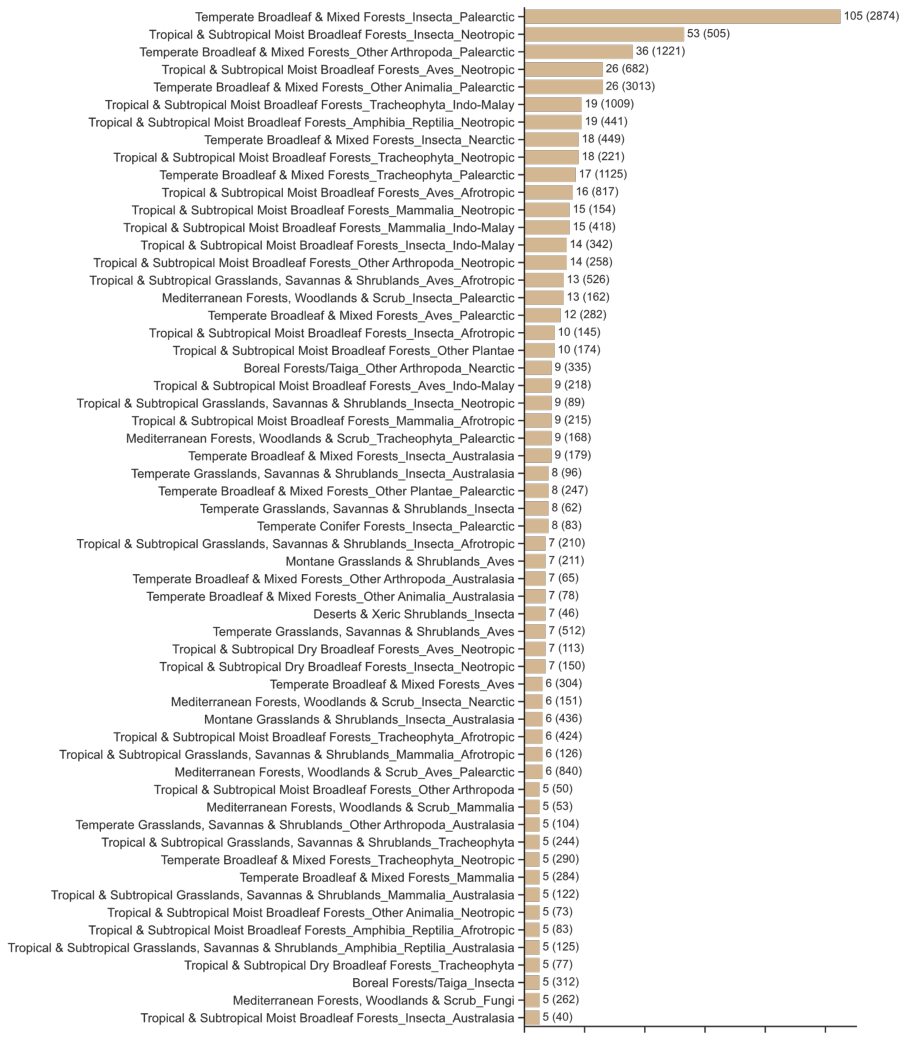
\includegraphics[width=0.95\linewidth]{figures/extended/hierarchical_groups.pdf}
    \caption{
    \textbf{Hierarchical groups in the BTMs.}
    Number of source studies and sampling sites (in parenthesis) in each final biogeographic-taxonomic group included in the BTMs. Some groups are at the biome-taxonomy-realm level, while others have been rolled up to the biome-taxonomy level. Groups that were rolled up to the overall population mean level have been excluded.}
    \label{fig:hierarchical_groups}
\end{extendedfigure}
\newpage

\begin{extendedfigure}[H]
    \centering
    \noindent\rule{\linewidth}{0.4pt}\par\vspace{6pt}
    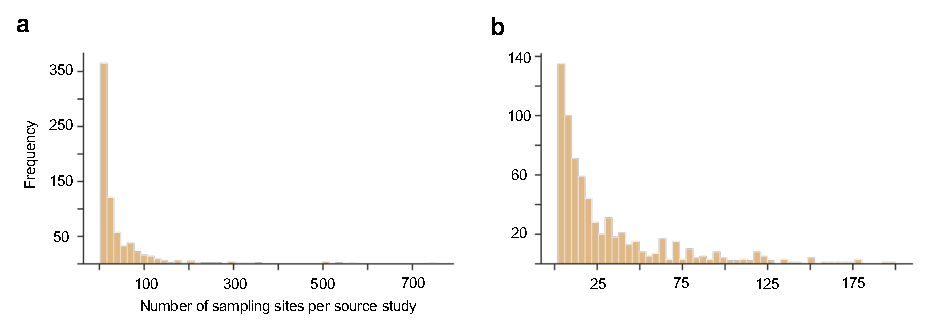
\includegraphics[width=0.95\linewidth]{figures/extended/sites_per_study.pdf}
    \caption{
    \textbf{Sampling sites per study.}
    \textbf{a}, Distribution over the number of sampling sites per source study in the analysis. \textbf{b}, The same distribution but capped at 200 sites, to better show the distribution of the majority of source studies. In the data, 18.8\% of studies have 5 sites or less, while 60.9\% have 25 or less.}
    \label{fig:sites_per_study}
\end{extendedfigure}
